% !TeX spellcheck = en_US
% !TeX root = ./0_article.tex

\section{Modeling and simulating BBI}
\IEEEPARstart{S}{imulating} a fault injection method behavior is an important part in understanding its mechanisms.
Whether it is EMFI, LFI or BBI, it allows to predict and understand the underlying phenomena at work to set up reliable experiments.
In this paper, we are focusing solely on BBI.

Ideally, we would want to directly observe signals inside integrated circuits, allowing for fine measurements of power supply voltages, logic levels and power current not to cite every physical quantity.
However, embedding sensors into an already existing IC is not possible, and doing so on future IC is costly and takes time to fully implement.
In addition to this, we do not have any guarantee that these sensors will not be disturbed too much by the fault injection.
Therefore, we have decided to take the following approach:
\begin{center}
	Simulation \textrightarrow\ Conclusions \textrightarrow\ Verification
\end{center}

By doing so, we have freed ourselves from hardware limitations.
However, other limitations remains.
Indeed, modern ICs, even the smallest, embed millions of transistors, and with current technologies, it is impossible to evaluate with simulations entire circuits at a transistor level.
Therefore, to tackle these limitations, we decided to adopt an hybrid approach, combining transistor-less models and local logic gates simulations.
This approach is a compromise between accuracy and computational cost/time, and allows simulating relatively big circuits under BBI disturbances
Overall, it is similar to what has been done for EMFI in \cite{mathieuEMFI}.
The resulting simulation flow is divided in three consecutive steps:
\begin{itemize}
	\item The simulation of an IC under BBI using a transistor-less model, allowing for a purely electrical analysis;
	\item The extraction of significant disturbed signals from the previous simulation;
	\item The simulation of functional logic gates under BBI thanks to the previously extracted signals.
\end{itemize}

\subsection{An hybrid simulation flow: building the models}
	Building the correct models for the simulation flow pass through multiple steps.
	As the goal of the hybrid flow is to reduce the computational power required to evaluate an IC, it is still important to maintain a certain accuracy concerning the IC physical structure.
	To do so, the models are designed around actual IC implementations.
	The main building blocks of the models are the power supply network, the standard-cells, and the substrate structure.
	In this work, we are only focusing on bulk substrates: specifically dual-well and triple-well substrates.

	\subsubsection{Power supply rails and standard-cell segments}
		% !TeX spellcheck = en_US
% !TeX root = ./0_article.tex
% LABEL AFTER CAPTION WESH GEOFFREY !!
\begin{figure}[h]
	\centering
	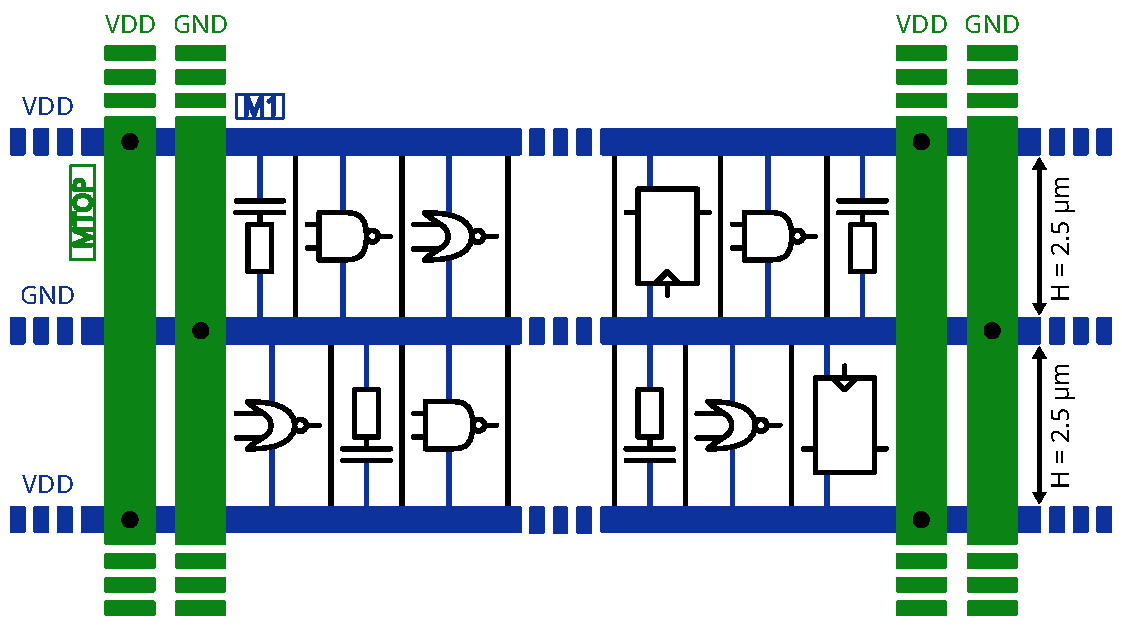
\includegraphics[width=0.49\textwidth]{./figures/psu_std_cell.pdf}
	\caption{A Standard-Cell Segment and its power delivery network.}
	\label{fig_alim_std}
\end{figure}

		The power distribution inside an IC is typically made with a grid-like structure, composed of metal wires stacked on top of each other on planes.
		In each layer, the metal wires are equally spaced and have a dedicated width, which becomes thinner the deeper they are.
		The lowest layer brings the power directly to the transistors.
		Fig. \ref{fig_alim_std} presents a common power delivery network, designed with two metal levels for simplicity.

		Within the metal lines are located standard-cell segments (SCS), composed of decoupling, logic and sequential elements, and are pre-characterized by foundries and categorized depending on their performance (mainly but not exclusively power consumption and speed).
		As illustrated in Fig. \ref{fig_alim_std}, SCS have a constant height, in our case of 2.5 \textmu m, and a variable width depending on how much logic gates each one of them embed.
		As we have stated previously, the hybrid simulation flow use transistor-less models as basic IC building blocks.
		Therefore, the transistors, hence the standard-cell segments, are modeled with passive elements such as resistors and capacitors.

		% !TeX spellcheck = en_US
% !TeX root = ./0_article.tex

\begin{figure}[h]
	\centering
	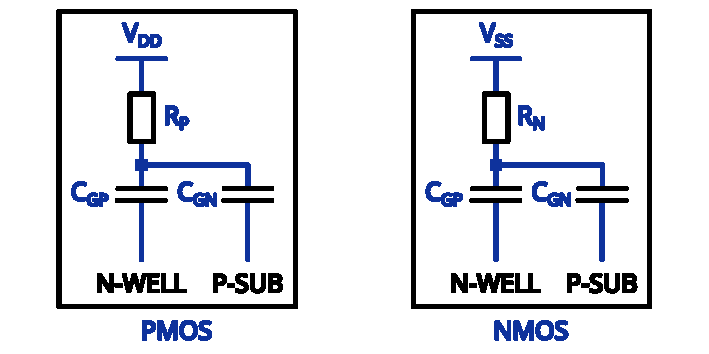
\includegraphics[width=0.9\columnwidth]{./figures/std_cell_logic_passive.pdf}
	\caption{Transistor-less equivalent model of a set of PMOS and NMOS in a SCS.}
	\label{mos_passive}
\end{figure}

		To that end, the elementary SCS chosen measures 30 \textmu m by 5 \textmu m, representing two rows of logic cells.
		This represents about a hundred of logic gates, represented with four resistors and two capacitors, as shown in Fig. \ref{mos_passive}, with half of the transistors conducting, half not conducting.
	%	Respectively, the conducting NMOS and PMOS transistors, whose source is respectively connected to $V_{SS}$ and $V_{DD}$ are respectively equivalent to a passive resistor $R_N$ and $R_P$.
		The conducting NMOS transistors, whose source is connected to $V_{SS}$, are equivalent to the passive resistor $R_N$.
		The conducting PMOS transistors, whose source is connected to $V_{DD}$, are equivalent to the passive resistor $R_P$.
		The resistors values depends on the considered technology, as well as the capacitors values, and can be adjusted and calculated according to one needs.

	\subsubsection{The substrate}
		% !TeX spellcheck = en_US
% !TeX root = ./0_article.tex

\begin{figure}[h]
	\centering
	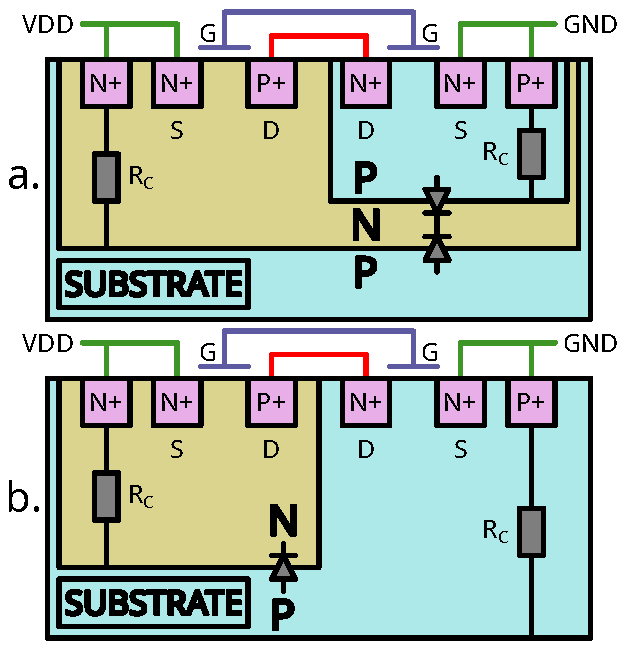
\includegraphics[width=0.35\textwidth]{./figures/substrate_2.pdf}
	\caption{Triple-well (a) and Dual-well (b) inverter cross-sectional view.}
	\label{fig_sub}
\end{figure}

		Because BBI can be performed thanks to the silicon substrate as the main physical environment transferring energy from a generator to an IC, it is fundamental to elaborate a proper substrate model to precisely represent the various involved phenomena.
		As stated previously, our work focuses on bulk substrates, and in most cases, the substrate silicon is P-doped.
		There are two typical ways of lithographing the transistors in a bulk substrate, using dual-well or triple-well structures.
		Dual-well substrates are commonly found in moderately old circuits, while triple-well substrates are found in more recent circuits, while not bleeding-edge.

		To properly understand how the differences between dual-well and triple-well substrates change the resulting model, let us analyze the cross-sectional schematics of an inverter created respectively in a triple-well and a dual-well substrate, as shown respectively in Fig. \ref{fig_sub}.a and Fig. \ref{fig_sub}.b:
		\begin{itemize}
			\item In the triple-well substrate, the NMOS transistors are lithographed into a P-doped silicon well, itself lithographed inside a N-doped well, buried inside the P-doped substrate. The PMOS transistors are located inside the N-doped well;
			\item In the dual-well substrate, the PMOS transistors are still located inside the N-doped well, however, the NMOS are lithographed directly inside the P-doped substrate.
		\end{itemize}
		On the one hand, the triple-well substrate reveals two diodes:
		\begin{itemize}
			\item One formed between the P-well and the N-well;
			\item Another formed between the N-well and the P-substrate.
		\end{itemize}
		On the other hand, the dual-well substrate only reveals one diode between the N-well and the P-substrate.

	\subsubsection{The resulting model}
		Thanks to what we have introduced previously, we can now build the elementary building blocks for our hybrid simulation flow.
		It combines the power delivery network architecture, the equivalent logic gates models, and the substrate structure, all in an embedded model.
		This model represents an elementary section of the simulated IC, measuring 30 \textmu m by 5 \textmu m by $t_{Sub}$ \textmu m, the latter being the substrate thickness, a parameter which will vary depending on each considered IC.
		% !TeX spellcheck = en_US
% !TeX root = ./0_article.tex

\begin{figure*}[ht]
	\centering
	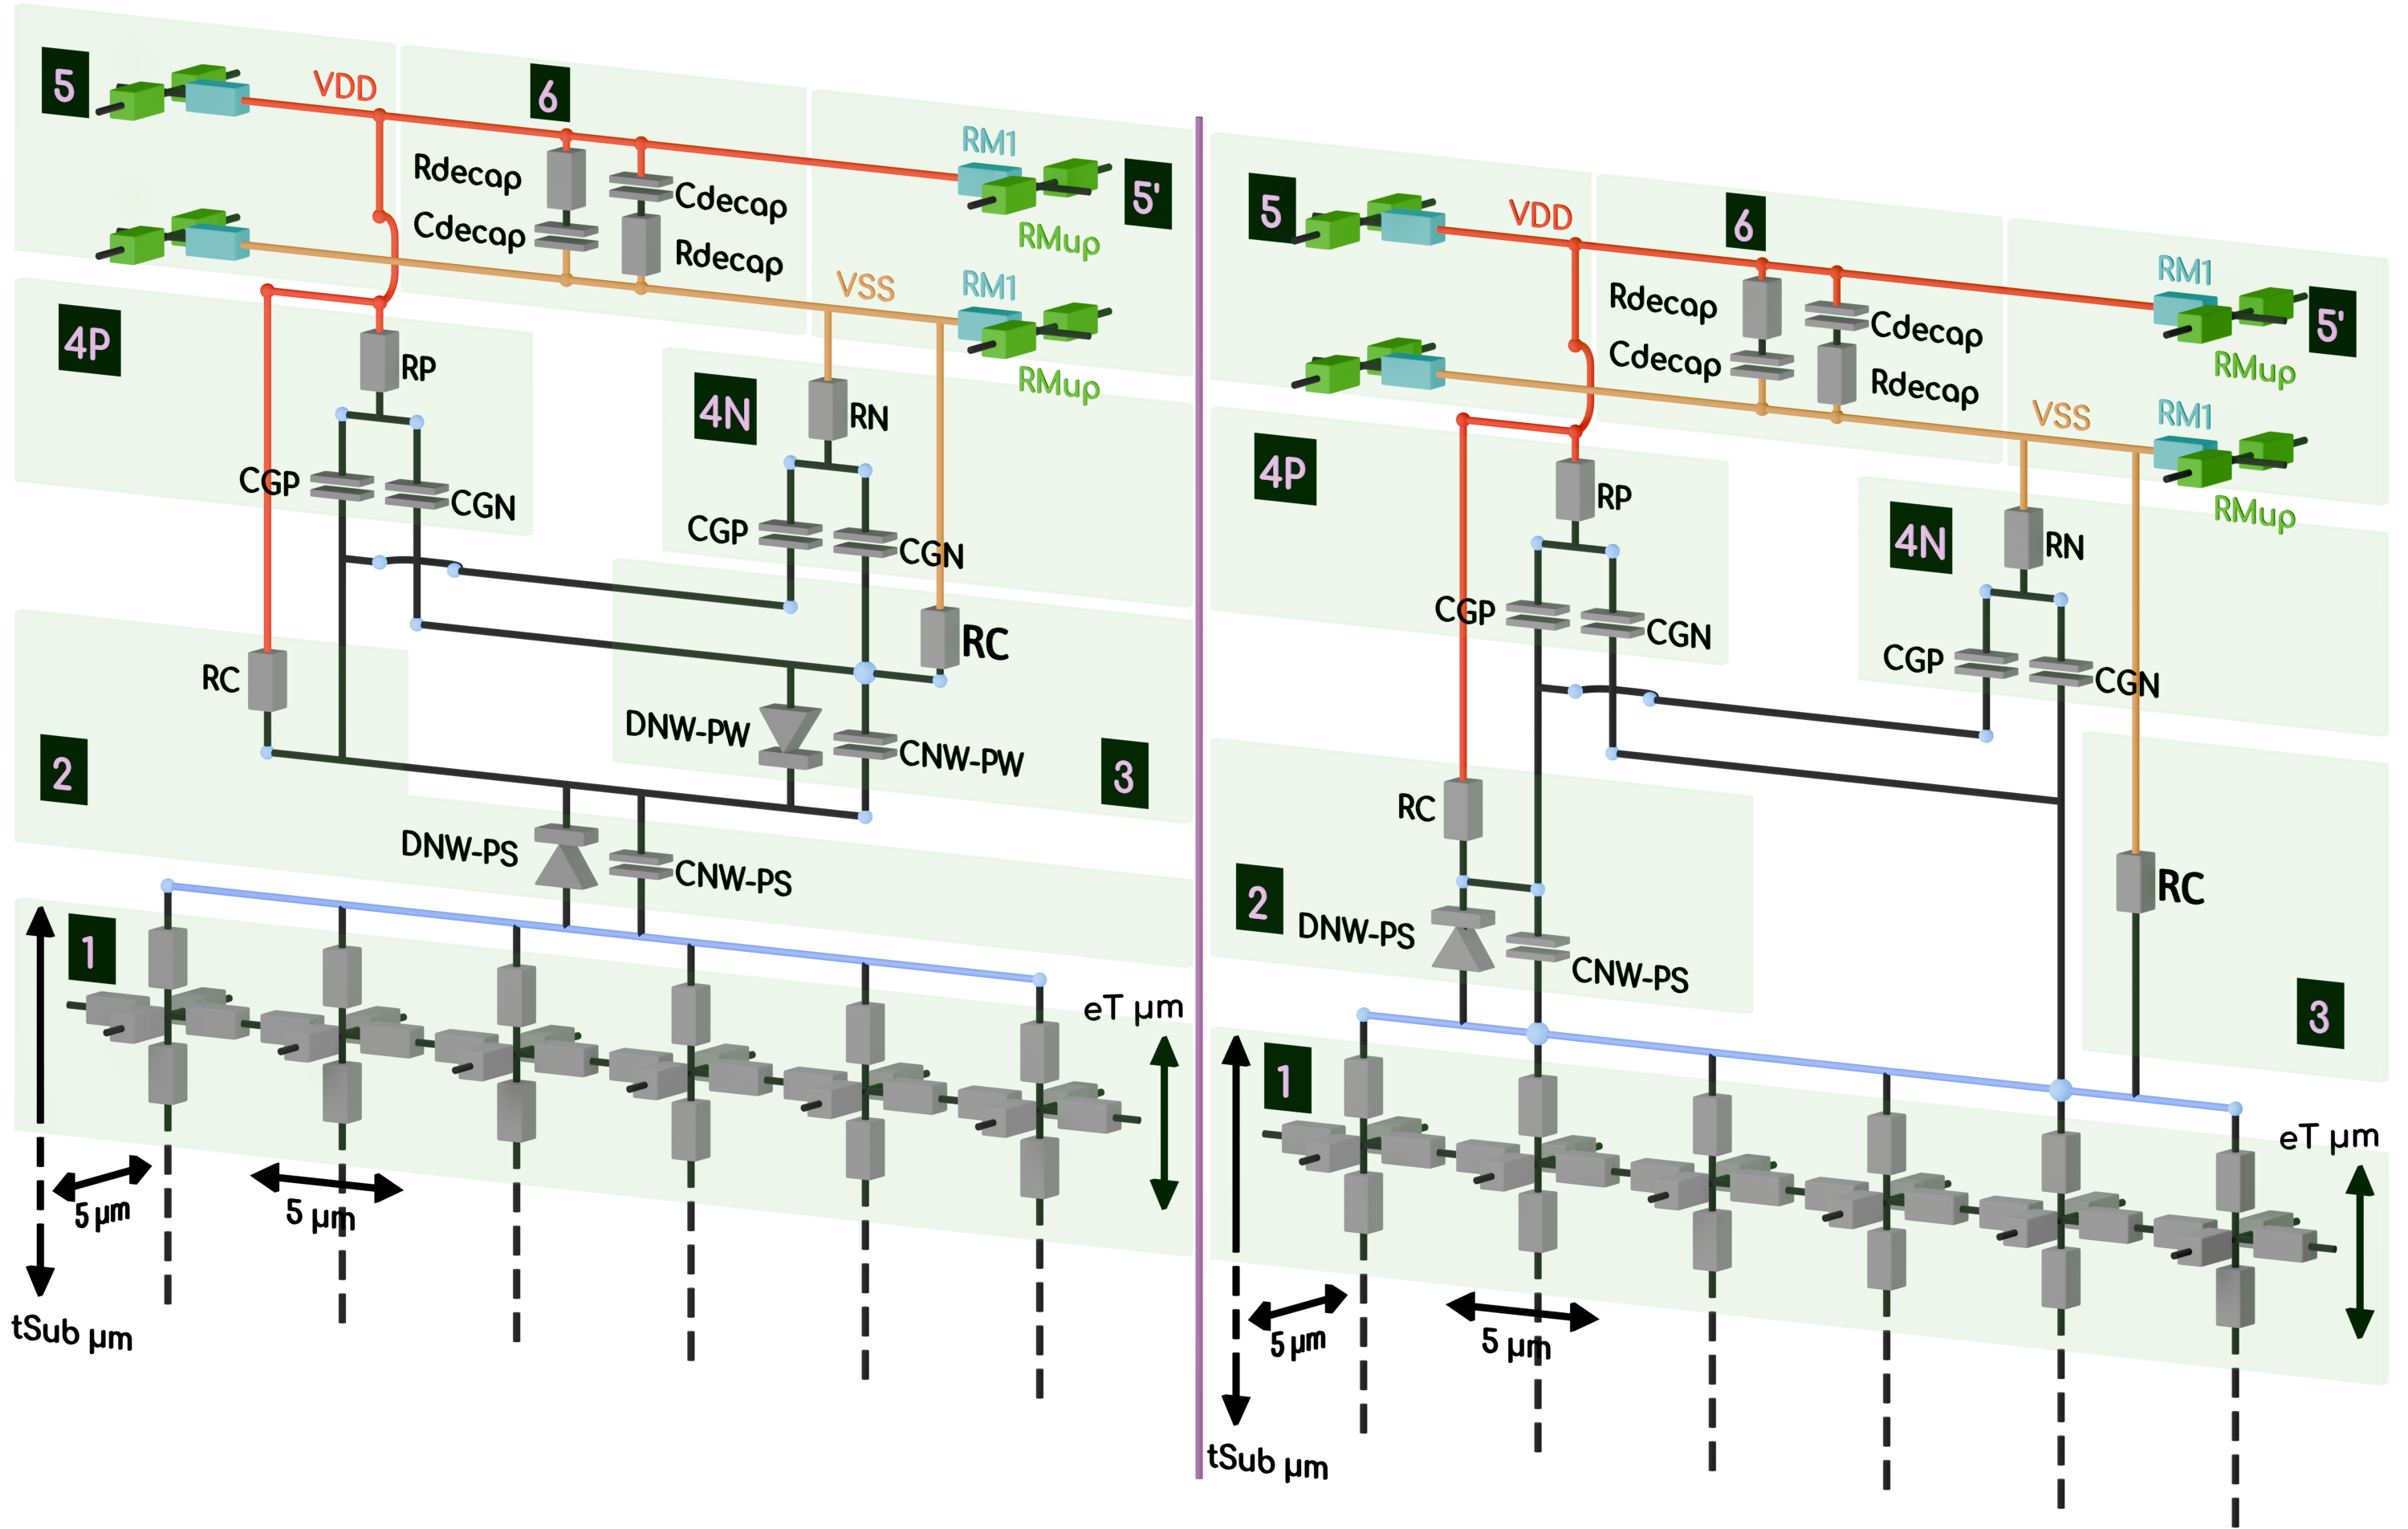
\includegraphics[width=0.95\textwidth]{./figures/dual+triple3.png}
	\caption{Triple well (left) and dual well (right) std cell \textcolor{red}{(PEUT ETRE FAIRE DES SOUS-FIGURES)}}
	\label{fig_triplewellstdcell}
\end{figure*}

		As we consider both triple-well and dual-well substrate, there are two resulting elementary models, shown in Fig. \ref{fig_triplewellstdcell}.
		Each model is composed of various sub-regions, whose descriptions follow:
		\begin{itemize}
			\item \ovalbox{1} is the substrate network, divided into six sub-networks of six resistors for finer details;
			\item \ovalbox{2} is the first P-N silicon junction, common to both models;
			\item \ovalbox{3} is the access resistor (DW) or the second junction (TW);
			\item \ovalbox{4P} is the PMOS equivalent section;
			\item \ovalbox{4N} is the NMOS equivalent section;
			\item \ovalbox{5, 5'} are the power supply metal layers (upper metal in green, first level in blue);
			\item \ovalbox{6} is the power supply decoupling.
		\end{itemize}
		As we have stated before, these models only represent a small portion of the modeled IC.
		To create an entire IC of a defined size, it is required to instantiate and interconnect as much as needed the elementary models.
		By doing so, we can create a bigger model of virtually any size.
		The language we have chosen to work with the simulation is the SPICE language.
		However, we created a custom Python script to interconnect the SCS together and generate a generic SPICE file.

\subsection{An hybrid simulation flow: performing simulations}
	Now that we set up the base models and their duplication, we can perform simulations with those models.
	To properly use these models, it is required, in the first place, to validate them through various steps to ensure their reliability.
	To that end, we generated an IC measuring 600 \textmu m by 600 \textmu m with a 200 \textmu m substrate thickness, and performed an operating point to verify the correctness of the models for each substrate type.
	% !TeX spellcheck = en_US
% !TeX root = ./0_article.tex

\begin{table}[H]
	\label{tab_op}
	\centering
	\begin{tabular}{lll}
		Value  & Triple-well & Dual-well \\ \hline
		$I_{GND}$                               & 2 nA          & 2.2 nA    \\
		$I_{VDD}$                                & -7 nA        & 3 nA        \\
		$\overline{GND_{drop}}$    & 2 nV         & 2 nV        \\
		$\overline{V_{DD_{drop}}}$    & 3 nV         & 3 nV       
	\end{tabular}
	\caption{op point}
\end{table}

	We should expect almost no voltage drop and zero current consumption from such a model.
	Otherwise, it indicates an underlying issue with the model.
	
	Table \ref{tab_op} shows the operating point results for both a triple-well and a dual-well circuit, and indicates a correct operating point.
	However, verifying the bias point alone is not sufficient to consider the model validated.
	As these models are dedicated to be mainly used in transient simulations, it is required to perform one and evaluate the soundness of its results.